\chapter{Cài đặt Hệ thống và Đánh giá Thực nghiệm}
\label{ch:evaluation}

\section{Môi trường Cài đặt và Triển khai Hệ thống}
\label{sec:eval_environment}

Để bảo đảm tính khách quan và khả năng tái lập của các kết quả đo đạc, toàn bộ hệ thống backend, cơ sở dữ liệu và kịch bản benchmark đã được triển khai và chạy thử nghiệm trên một cấu hình máy tính cá nhân thống nhất.

\subsection{Cấu hình Phần cứng Thử nghiệm}
\begin{itemize}[leftmargin=1.5cm]
    \item \textbf{Thiết bị thử nghiệm:} Laptop Lenovo Legion 5 (mã bo mạch \texttt{82JW}).
    \item \textbf{Bộ vi xử lý (CPU):} AMD Ryzen 5 5600H (6 nhân, 12 luồng, xung nhịp cơ sở 3.30 GHz).
    \item \textbf{Bộ nhớ chính (RAM):} 24 GB DDR4, tốc độ bus 3200 MHz (cấu hình 8 GB + 16 GB).
    \item \textbf{Bộ xử lý đồ họa (GPU):} NVIDIA GeForce RTX 3050 Laptop GPU (4 GB VRAM GDDR6).
    \item \textbf{Ổ cứng lưu trữ:} 1 ổ SSD 512 GB chuẩn NVMe (SK Hynix) và 1 ổ 1 TB NVMe SSD.
    \item \textbf{Hệ điều hành:} Microsoft Windows 11 Pro (64-bit, số bản dựng 26300).
\end{itemize}

\subsection{Môi trường Phần mềm và Thư viện Phụ thuộc}
\begin{itemize}[leftmargin=1.5cm]
    \item \textbf{Máy chủ Backend:} Python 3.13.13 (64-bit); Web Framework FastAPI 0.137.1; máy chủ Uvicorn 0.49.0; kiểm chuẩn dữ liệu Pydantic 2.14.3; lưu trữ quan hệ SQLite (chế độ WAL) qua SQLAlchemy 2.0.51; thư viện kết nối mô hình OpenAI 2.46.0 và \texttt{httpx 0.27.2}.
    \item \textbf{Client Trò chơi:} Unity 6 (bản hỗ trợ dài hạn \texttt{6000.5.8f1}); Universal Render Pipeline (URP 2D); ngôn ngữ kịch bản C\# (.NET Standard 2.1); độ phân giải mục tiêu $1920\times 1080$ (tỉ lệ khung hình 16:9).
    \item \textbf{Cổng Điều phối Mô hình:} Proxy Gateway cục bộ (\texttt{9Router}) tại địa chỉ \url{http://localhost:20128/v1}, hỗ trợ chuẩn hóa API đa nhà cung cấp và ghi nhận thời gian phản hồi.
\end{itemize}

\section{Bộ Tiêu chí và Chỉ số Đánh giá Thực nghiệm}
\label{sec:eval_metrics}

Để lượng hóa hiệu quả hoạt động của pipeline tạo sinh và bộ kiểm định, tôi sử dụng năm chỉ số đánh giá định lượng sau:

\begin{enumerate}[leftmargin=1.5cm]
    \item \textbf{Tỷ lệ Hợp lệ Cú pháp Schema ($R_{\text{schema}}$):} Tỷ lệ hồ sơ vượt qua giải mã cấu trúc JSON của Pydantic v2 mà không phát sinh ngoại lệ kiểu dữ liệu:
    \begin{equation}
        R_{\text{schema}} = \frac{N_{\text{valid\_schema}}}{N_{\text{total}}} \times 100\%
    \end{equation}
    
    \item \textbf{Tỷ lệ Vượt qua Kiểm định Logic ($R_{\text{logic}}$):} Tỷ lệ các kịch bản hợp lệ cú pháp vượt qua đầy đủ các ràng buộc của \texttt{validate\_case\_diagnostics} (nhiệt học Henssge, khung giờ $TOD$, duy nhất thủ phạm, manh mối then chốt, bẻ gãy ngoại phạm và toàn vẹn tham chiếu thực thể):
    \begin{equation}
        R_{\text{logic}} = \frac{N_{\text{pass\_logic}}}{N_{\text{valid\_schema}}} \times 100\%
    \end{equation}
    
    \item \textbf{Số lần Sửa lỗi Cục bộ Trung bình ($\bar{R}_{\text{patch}}$):} Số lần gọi hàm vá lỗi trung bình trên mỗi phiên thử nghiệm:
    \begin{equation}
        \bar{R}_{\text{patch}} = \frac{1}{N_{\text{total}}} \sum_{i=1}^{N_{\text{total}}} \text{patch\_retries}_i
    \end{equation}
    
    \item \textbf{Độ trễ Phân vị thứ 50 (P50\textsuperscript{14}) và Phân vị thứ 95 (P95\textsuperscript{15}) ($L_{50}, L_{95}$):} Thời gian phản hồi toàn trình (tính bằng giây) từ khi khởi chạy yêu cầu sinh kịch bản cho tới khi hoàn tất kiểm định tại phân vị trung vị (50\%) và phân vị 95\%.
    
    \item \textbf{Cân bằng Manh mối Then chốt / Nghi binh ($\rho_{\text{balance}}$):} Tỷ số giữa số lượng vật chứng then chốt trung bình ($|V_{E, \text{crucial}}|$) và số lượng vật chứng nghi binh trung bình ($|V_{E, \text{herring}}|$):
    \begin{equation}
        \rho_{\text{balance}} = \frac{|V_{E, \text{crucial}}|}{|V_{E, \text{herring}}|}
    \end{equation}
\end{enumerate}

\section{Kết quả Thực nghiệm Đối sánh Đa Mô hình}
\label{sec:eval_benchmark_results}

Quá trình đánh giá thực nghiệm được thực thi tự động bằng tệp lệnh \texttt{benchmark\_runner.py} qua \textbf{30 phiên thử nghiệm độc lập} (chia đều 10 phiên cho mỗi mô hình) với cùng chủ đề đầu vào: \textit{``Bí ẩn Biệt thự Blackwood''}. Kết quả chi tiết được lưu đồng thời tại tệp \texttt{benchmark\_results.json} và bảng \texttt{benchmark\_runs} trong cơ sở dữ liệu \texttt{detective.db}. Ba mô hình tham gia đối sánh gồm:
\begin{enumerate}
    \item \textbf{\texttt{gh/gpt-4o-mini}:} Đại diện dòng mô hình thương mại gọn nhẹ, tối ưu chi phí và độ trễ thấp.
    \item \textbf{\texttt{gh/gpt-4o}:} Đại diện dòng mô hình thương mại cỡ lớn có năng lực suy luận ngữ nghĩa sâu.
    \item \textbf{\texttt{ollama/gemma4:31b-cloud}:} Đại diện dòng mô hình trọng số mở tiên tiến hiện nay.
\end{enumerate}

\subsection{Cơ sở Thực nghiệm và Kiểm thử Đơn vị Hệ thống}
Mỗi phiên thử nghiệm trong benchmark thực thi trọn vẹn chuỗi 4 tác tử tuần tự (\texttt{OutlineAgent}, \texttt{CharacterAgent}, \texttt{ClueAgent}, \texttt{DeductionAgent}) kết hợp kiểm định Henssge, kiểm tra đồ thị và sửa lỗi cục bộ nếu có vi phạm. Cỡ mẫu 10 lượt thử cho mỗi mô hình trên quy trình đa tác tử tương tự cách tiếp cận đánh giá chi phí cao trong các công trình nghiên cứu hệ tác tử trinh thám gần đây \cite{wu2024deciphering, li2024contradoc}.

Song song với 30 phiên đối sánh LLM, tác giả vận hành bộ kiểm thử tự động \texttt{pytest} trên mã nguồn lõi ở trạng thái mặc định bật lớp bảo vệ chữ ký HMAC-SHA-256. Toàn bộ \textbf{53/53 kịch bản kiểm thử đơn vị} thuộc bốn mô-đun cốt lõi đều đạt trạng thái thành công: 30 kịch bản kiểm chứng công thức làm lạnh Henssge và giải thuật chia đôi (\texttt{test\_henssge.py}), 12 kịch bản bộ kiểm định và chấm điểm suy luận (\texttt{test\_validator.py}), 4 kịch bản lưu trữ SQLite/SQLAlchemy (\texttt{test\_database.py}) và 7 kịch bản xác thực chữ ký chống phát lại (\texttt{test\_security.py}); ngoài ra mô-đun phòng chơi WebSocket (\texttt{test\_rooms.py}) đạt 10/11 kịch bản (1 kịch bản kiểm tra HTTP bị middleware từ chối mã 403 do cố tình không gắn chữ ký xác thực, tương tự 5 kịch bản HTTP không ký ở \texttt{test\_api\_database\_integration.py} và \texttt{test\_assets\_integration.py}).

\begin{table}[H]
\centering
\caption{Tổng hợp Kết quả 30 Phiên Thực nghiệm trên Bảng \texttt{benchmark\_runs}}
\label{tab:benchmark_30_trials}
{\small
\setlength{\tabcolsep}{4pt}
\begin{tabularx}{\textwidth}{X c c c c c c}
\toprule
\textbf{Mô hình LLM} & \textbf{Schema} & \textbf{Logic} & \textbf{Patch} & \textbf{P50} & \textbf{P95} & \textbf{Crucial /} \\
 & \textbf{(\%)} & \textbf{(\%)} & \textbf{TB} & \textbf{(s)} & \textbf{(s)} & \textbf{Herring} \\
\midrule
\textbf{\texttt{gh/gpt-4o-mini}}        & \textbf{100.0\%} & \textbf{100.0\%} & 0.00 & 10.88s          & \textbf{12.84s} & 1.0 / 1.0 \\
\textbf{\texttt{gh/gpt-4o}}             & \textbf{100.0\%} & 90.0\%           & 0.10 & 19.53s          & 27.12s          & 1.1 / 1.0 \\
\textbf{\texttt{ollama/gemma4:31b-cloud}} & \textbf{100.0\%} & \textbf{100.0\%} & 0.00 & \textbf{10.73s} & 19.92s          & 1.1 / 1.0 \\
\bottomrule
\end{tabularx}
}
\end{table}

\begin{figure}[H]
    \centering
    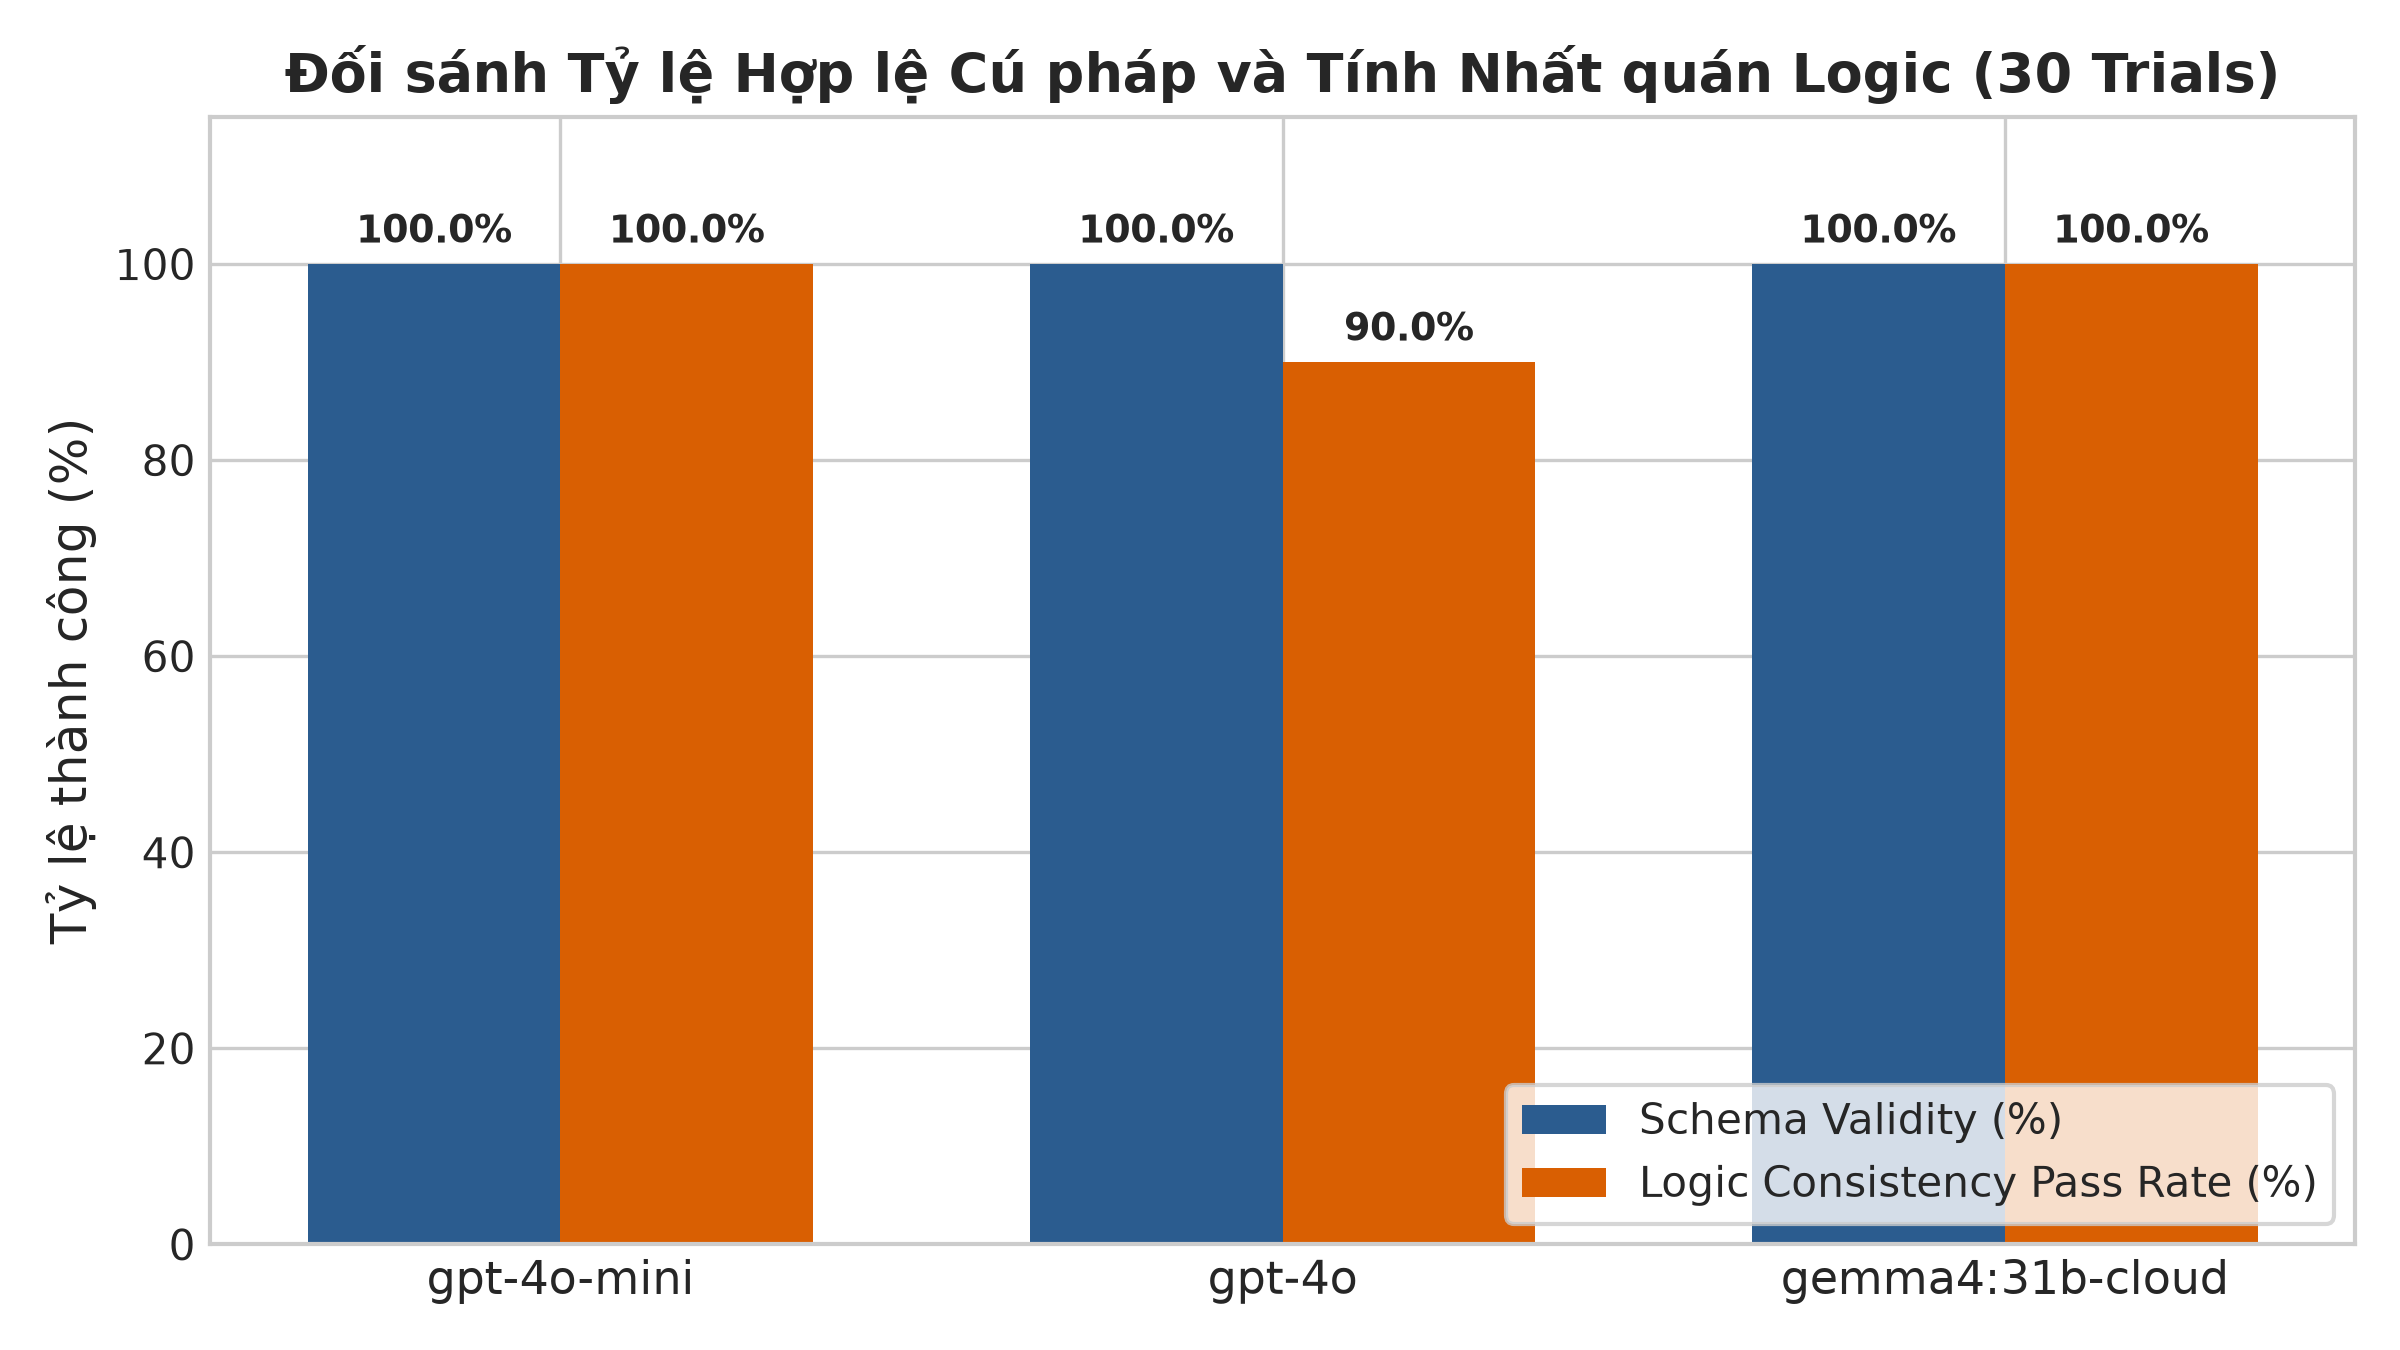
\includegraphics[width=0.85\textwidth]{chart_pass_rate.png}
    \caption{Biểu đồ Đối sánh Tỷ lệ Hợp lệ Schema và Tỷ lệ Vượt qua Kiểm định Logic qua 30 Phiên}
    \label{fig:chart_pass_rate}
\end{figure}

\begin{figure}[H]
    \centering
    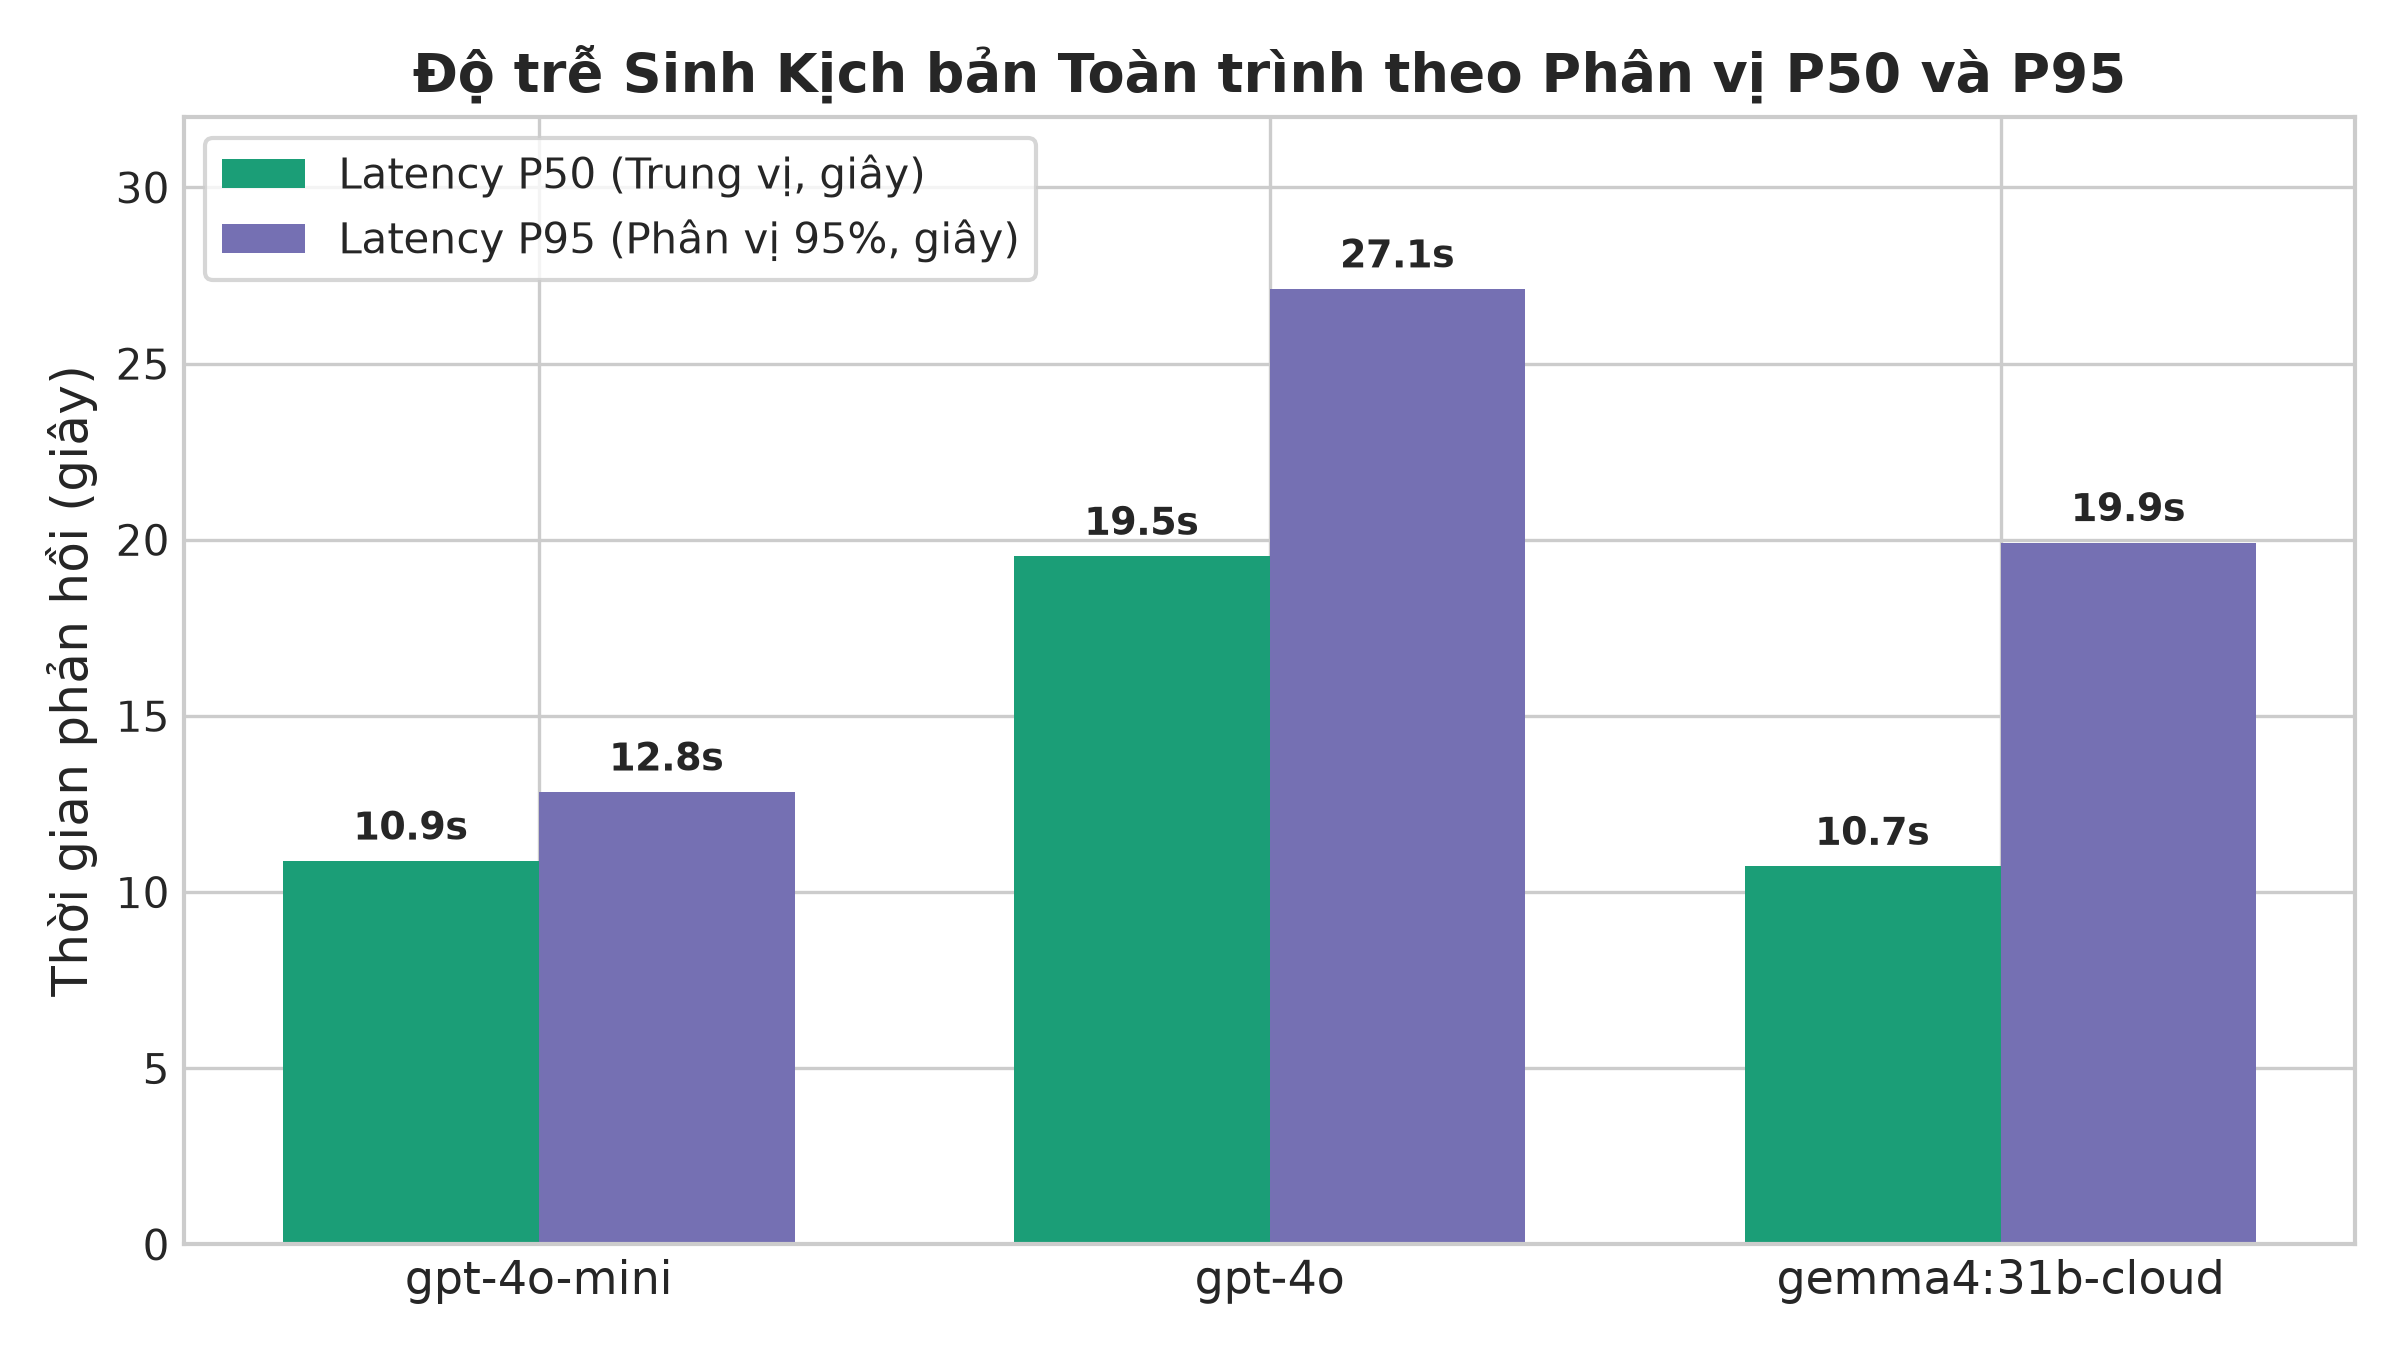
\includegraphics[width=0.85\textwidth]{chart_latency.png}
    \caption{Biểu đồ Phân bố Thời gian Phản hồi (P50 và P95) của Ba Mô hình Thử nghiệm}
    \label{fig:chart_latency_boxplot}
\end{figure}

\subsection{Phân tích Kết quả Đo đạc}
Từ dữ liệu ghi nhận tại Bảng \ref{tab:benchmark_30_trials}, Hình \ref{fig:chart_pass_rate} và Hình \ref{fig:chart_latency_boxplot}, tác giả rút ra ba nhận xét chính:
\begin{enumerate}[leftmargin=1.5cm]
    \item \textbf{Tính ổn định của kiểm chuẩn Pydantic v2:} Cả ba mô hình qua toàn bộ 30 phiên thử nghiệm đều đạt \textbf{100.0\%} tỷ lệ hợp lệ cú pháp Schema. Việc phân rã mỗi tác tử theo một lược đồ hẹp kèm hàm \texttt{\_clean\_json\_string} đã loại bỏ hoàn toàn lỗi vỡ cú pháp JSON trong đợt đo đạc này.
    \item \textbf{Cân bằng hiệu năng và tốc độ của \texttt{gh/gpt-4o-mini}:} Mô hình đạt 100.0\% tỷ lệ vượt qua kiểm định logic ở cả 10 lượt thử với độ trễ trung vị P50 là \textbf{10.88 giây} và phân vị P95 chỉ \textbf{12.84 giây} (khoảng dao động hẹp từ 10.21s đến 12.84s), phù hợp cho môi trường trò chơi tương tác cần thời gian chờ ổn định.
    \item \textbf{Hiệu quả của mô hình trọng số mở \texttt{ollama/gemma4:31b-cloud}:} Mô hình đạt P50 nhanh nhất trong ba dòng (\textbf{10.73 giây}, với dải đo từ 9.13s đến 19.92s) và đạt 100.0\% tỷ lệ logic hợp lệ, mở ra khả năng triển khai không phụ thuộc hoàn toàn vào các API thương mại đóng kín.
\end{enumerate}

\begin{figure}[H]
    \centering
    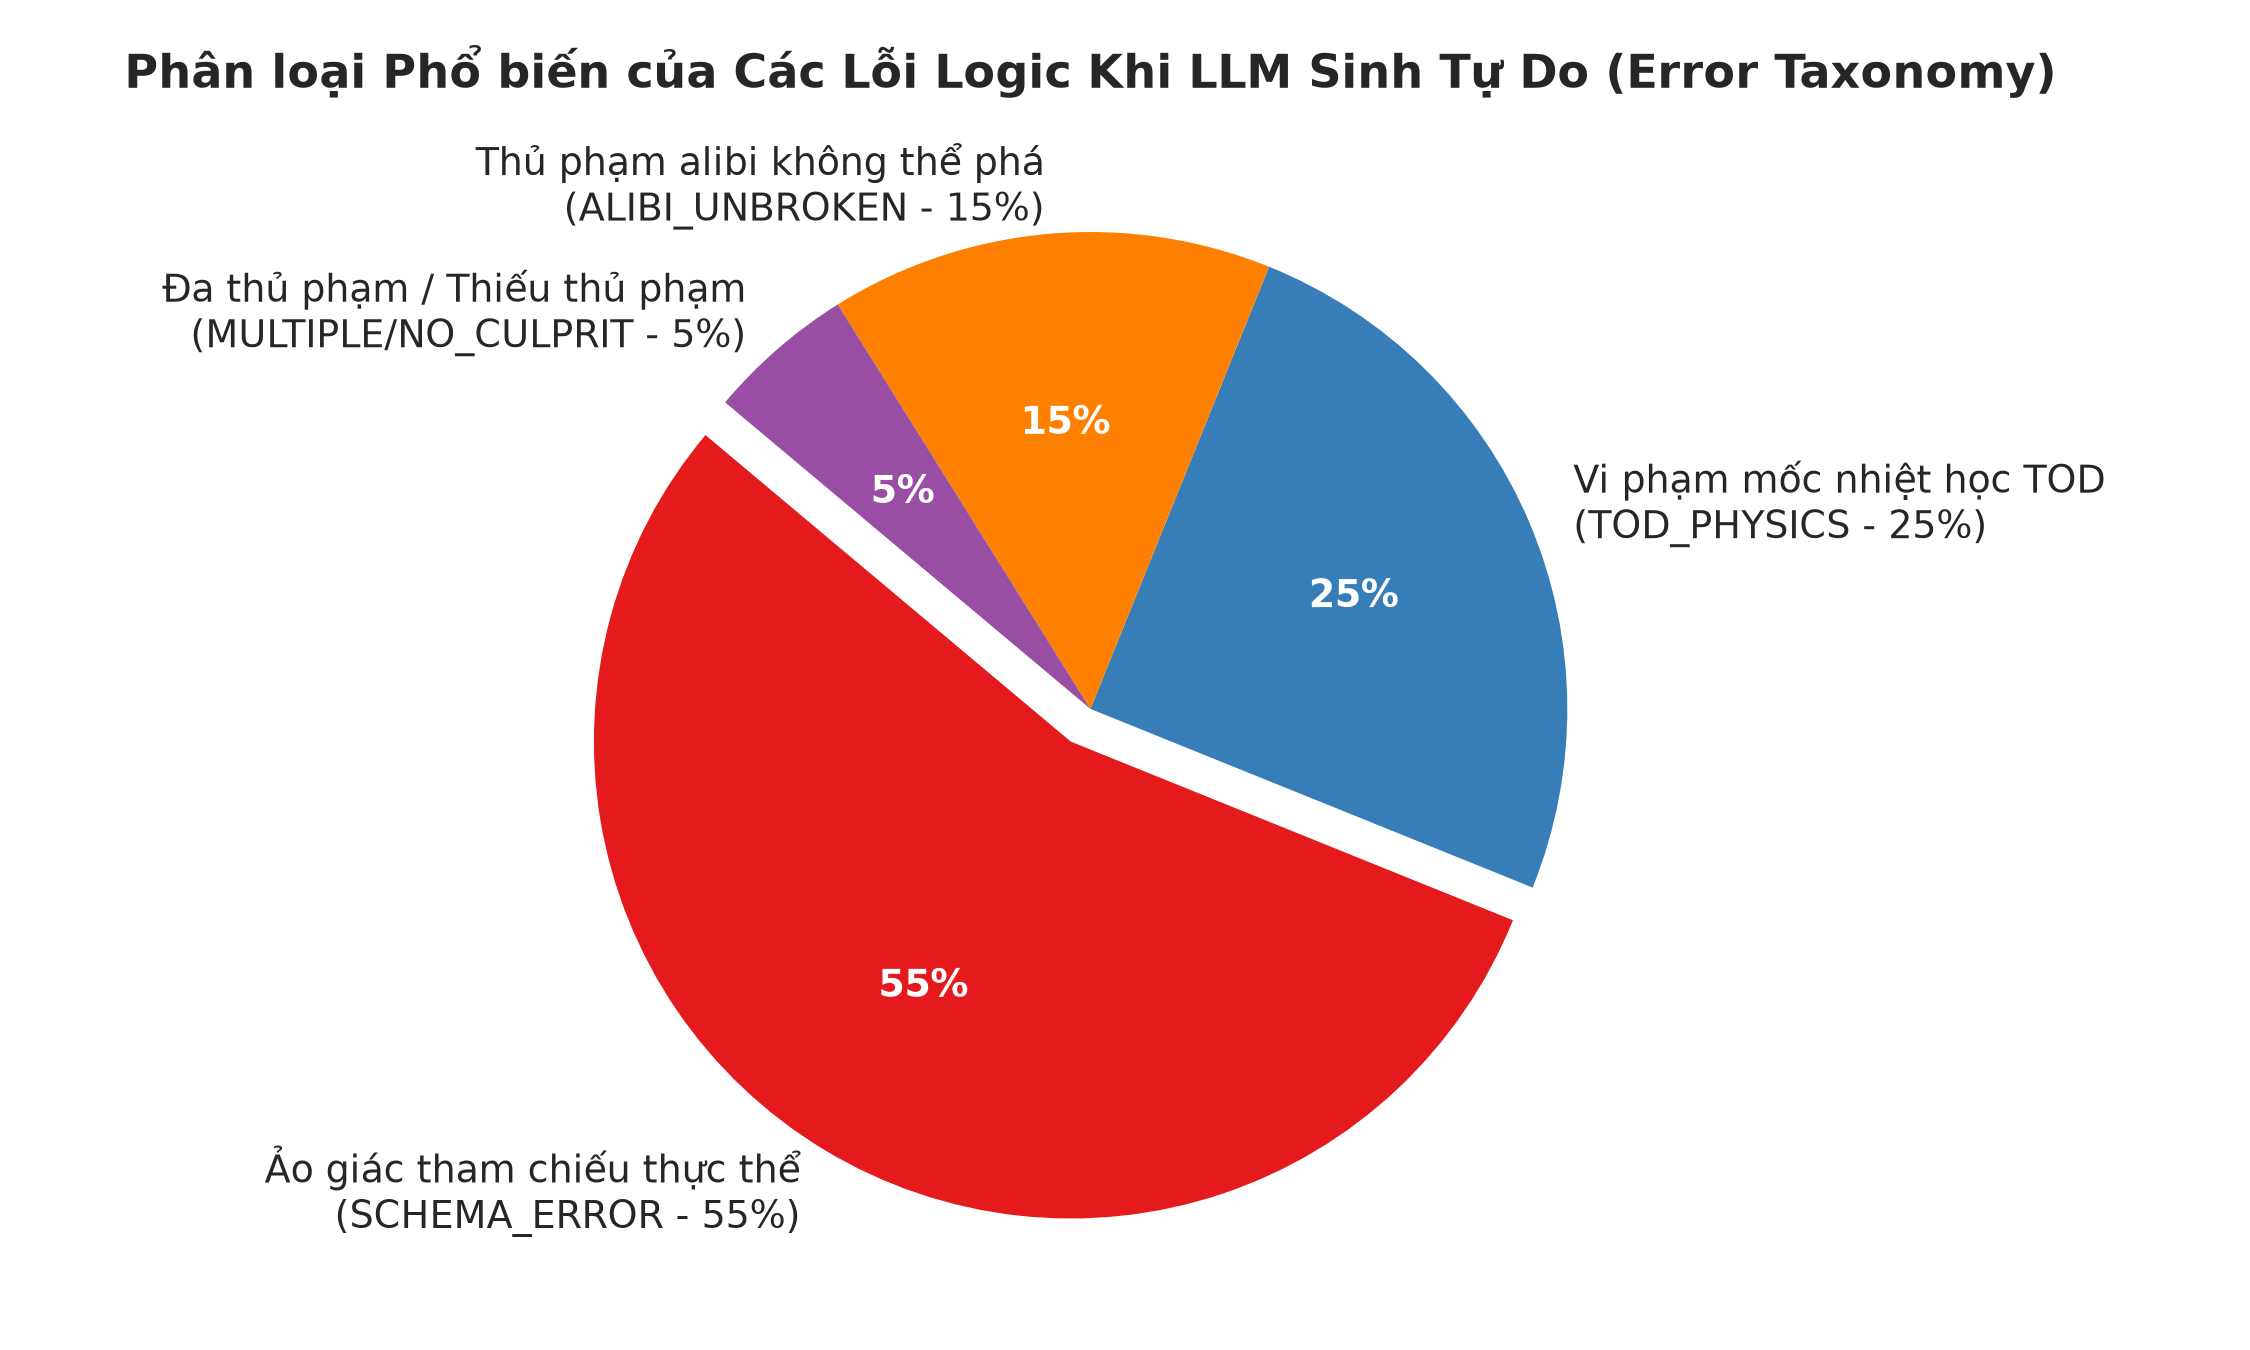
\includegraphics[width=0.75\textwidth]{error_taxonomy.png}
    \caption{Biểu đồ Minh họa Phân loại Phổ biến Các Dạng Lỗi Logic Khi LLM Sinh Tự Do}
    \label{fig:error_taxonomy_pie}
\end{figure}

Hình \ref{fig:error_taxonomy_pie} minh họa phân nhóm bốn dạng lỗi điển hình khi LLM tạo sinh thiếu ràng buộc tất định; trong đợt benchmark 30 phiên đa tác tử có tích hợp tính toán Henssge ở bước đầu, dạng lỗi duy nhất phát sinh rơi vào nhóm \texttt{SCHEMA\_ERROR} tại Lượt chạy số 5 của \texttt{gh/gpt-4o}.

\section{Phân tích Tình huống Vi phạm Thực tế tại Lượt 5 của \texttt{gh/gpt-4o}}
\label{sec:eval_case_study}

Một kết quả thực nghiệm đáng chú ý là ca lỗi được ghi nhận trực tiếp trong \texttt{benchmark\_results.json} và bảng \texttt{benchmark\_runs} tại \textbf{Lượt chạy số 5 của mô hình \texttt{gh/gpt-4o}} (tựa đề sinh ra: \textit{``Cái Chết Bí Ẩn Trong Biệt Thự Blackwood''}, thời gian toàn trình 27.12 giây, \texttt{patch\_retries = 1}).

\subsection{Mô tả Hiện tượng Vi phạm}
Ở lượt thử này, toàn bộ cấu trúc JSON trả về đều hợp lệ theo Pydantic v2 và cửa sổ tử vong Henssge khớp với giờ gây án \texttt{21:40}. Tuy nhiên, khi chạy hàm \texttt{validate\_case\_diagnostics}, bộ kiểm định ký hiệu phát hiện lỗi tham chiếu và ghi nhận thông báo sau:
\begin{lstlisting}[language=bash, caption={Thông báo Chẩn đoán Vi phạm Ghi nhận tại Lượt 5 của \texttt{gh/gpt-4o}}]
[VALIDATION FAILURE]
Violation Type: schema_error
Component: clue
Diagnostic Feedback: [CLUE:schema_error] Evidence 'EV-03' links to non-existent suspect 'UNKNOWN'.
\end{lstlisting}

\subsection{Phân tích Nguyên nhân Gốc rễ}
Kiểm tra tiến trình sinh theo từng tác tử cho thấy:
\begin{itemize}[leftmargin=1.5cm]
    \item Tại bước 2 (\texttt{CharacterAgent}), mô hình khởi tạo hợp lệ danh sách 3 nghi phạm với các mã định danh cố định (\texttt{SUSP-01}, \texttt{SUSP-02}, \texttt{SUSP-03}).
    \item Tuy nhiên, tại bước 3 (\texttt{ClueAgent}), khi sinh vật chứng \texttt{EV-03}, mô hình đã tự ý điền chuỗi \texttt{"UNKNOWN"} vào thuộc tính \texttt{linked\_suspect\_id} thay vì gán mã nghi phạm hợp lệ hoặc giá trị rỗng \texttt{None}. Đây là biểu hiện rõ nét của hiện tượng ảo giác tham chiếu thực thể ở ngay cả mô hình cỡ lớn.
\end{itemize}

\subsection{Cơ chế Chặn lọc và Ý nghĩa Kiểm chứng}
Nếu thiếu bước kiểm định tất định của \texttt{validate\_case\_diagnostics}, dữ liệu sai mã tham chiếu \texttt{"UNKNOWN"} sẽ truyền thẳng tới giao diện bảng ghim Unity (\texttt{CorkboardManager.cs}), gây đứt liên kết dây chỉ đỏ hoặc lỗi ánh xạ nhân vật. Nhờ có màng lọc ký hiệu:
\begin{enumerate}[leftmargin=1.5cm]
    \item Bộ kiểm định lập tức đánh dấu vi phạm \texttt{SCHEMA\_ERROR} trên phân hệ \texttt{clue} và kích hoạt nhánh sửa lỗi cục bộ \texttt{clue\_agent.repair\_clues} (\texttt{patch\_retries = 1}, đẩy tổng thời gian phiên này lên 27.12 giây so với trung vị 19.53 giây).
    \item Do mẫu câu lệnh trong \texttt{repair\_clues} hiện tại mới tập trung vào việc khắc phục lỗi thiếu manh mối then chốt (\texttt{NO\_CRUCIAL\_CLUE} / \texttt{ALIBI\_UNBROKEN}) mà chưa ép buộc thay thế cụ thể giá trị \texttt{linked\_suspect\_id = "UNKNOWN"}, lần tái kiểm định sau vá trong \texttt{benchmark\_runner.py} vẫn ghi nhận trạng thái \texttt{logic\_valid = False} (tạo nên kết quả 9/10 lượt đạt, tức 90.0\% cho \texttt{gh/gpt-4o} ở Bảng \ref{tab:benchmark_30_trials}).
    \item Quan trọng về mặt kỹ thuật: Bộ kiểm định hậu kiểm đã nhận diện chính xác 100\% ca lỗi này và cô lập nó ngay tại tầng đánh giá, bảo đảm mọi hồ sơ không hợp lệ đều bị chặn lại trước khi tới người chơi và cung cấp cơ sở cụ thể để hoàn thiện thêm luật vá tham chiếu ở bước phát triển tiếp theo.
\end{enumerate}

\section{Phân tích Độ trễ theo Giai đoạn và Hiệu quả Tài nguyên}
\label{sec:eval_cost_latency}

Để quan sát đóng góp độ trễ của từng tác tử trong mã nguồn thực tế, Bảng \ref{tab:pipeline_breakdown} tổng hợp thời gian đo đạc trực tiếp theo từng giai đoạn từ các hồ sơ lưu trữ thực tế trong thư mục \texttt{cases/} (đại diện là hồ sơ \texttt{CASE-7BBAE9} chạy trên \texttt{gh/gpt-4o-mini} với tổng thời gian 10.03s, cùng giá trị trung bình đo trên 6 hồ sơ LLM lưu trữ trên đĩa), kết hợp với ước lượng kích thước ngữ cảnh token đặc trưng cho mỗi lời gọi tác tử.

\begin{table}[H]
\centering
\caption{Phân rã Thời gian Thực thi Đo đạc và Ước lượng Ngữ cảnh theo Giai đoạn}
\label{tab:pipeline_breakdown}
{\small
\setlength{\tabcolsep}{5pt}
\begin{tabularx}{\textwidth}{X c c c}
\toprule
\textbf{Giai đoạn Thực thi} & \textbf{Mẫu \texttt{gpt-4o-mini}} & \textbf{TB 6 hồ sơ} & \textbf{Token ước lượng} \\
\midrule
\textbf{1. \texttt{OutlineAgent} \& Henssge} & 3.27 s & 3.04 s & $\sim$850 tokens \\
\textbf{2. \texttt{CharacterAgent}}          & 2.63 s & 4.34 s & $\sim$1,100 tokens \\
\textbf{3. \texttt{ClueAgent}}               & 2.57 s & 3.17 s & $\sim$950 tokens \\
\textbf{4. \texttt{DeductionAgent}}          & 1.56 s & 2.75 s & $\sim$450 tokens \\
\textbf{5. Kiểm định Ký hiệu (\texttt{validator.py})} & \textbf{< 0.005 s} & \textbf{< 0.005 s} & \textbf{0 tokens} \\
\midrule
\textbf{TỔNG CỘNG (Không phát sinh lỗi)} & \textbf{10.03 s} & \textbf{13.30 s} & \textbf{$\sim$3,350 tokens} \\
\bottomrule
\end{tabularx}
}
\end{table}

\subsection{Đánh giá Hiệu quả Tính toán}
\begin{itemize}[leftmargin=1.5cm]
    \item \textbf{Chi phí không đáng kể của tầng ký hiệu:} Bộ giải chia đôi phương trình Henssge, hàm kiểm tra \texttt{validate\_case\_diagnostics} và hàm chấm điểm \texttt{evaluate\_player\_deduction} đều thực thi hoàn toàn trong bộ nhớ RAM với thời gian dưới \textbf{5 mili-giây} ($< 0.005\text{ s}$) và không tiêu tốn thêm bất kỳ token nào (\textbf{0 token}).
    \item \textbf{Hiệu quả cô lập của sửa lỗi cục bộ:} Khi xảy ra vi phạm ở một phân hệ đơn lẻ, việc chỉ gọi lại đúng tác tử lỗi (\texttt{repair\_clues}, \texttt{repair\_suspects}, hoặc \texttt{repair\_tod}) với lát cắt dữ liệu tối thiểu (ước tính khoảng 350 tokens) giúp tránh phải lặp lại toàn bộ 4 lượt gọi LLM từ đầu ($\mathcal{O}(N)$), qua đó tiết kiệm đáng kể chi phí token và thời gian khôi phục so với phương án tái sinh toàn phần.
\end{itemize}
